\subsection{Rappel de la méthodologie utilisée}

Afin de simplifier les notations, dans la suite nous nous référons à 2 cas de méthodologie différentes nommées \og \textbf{individuel} \fg et \og \textbf{global} \fg. Cependant le nom choisi ne reflète pas entièrement la procédure, il faut donc bien garder en tête ce qu'on attend par ces noms de méthodologie :

\begin{table}[H]
	\centering
	\begin{tabularx}{\textwidth}{c|X|X}
		\toprule
		threshold/méthodologie & \textbf{individuel}                  & \textbf{global}                                                                                                                                                                                                               \\
		\bottomrule
		\\
		$\lambda < 110$        & $h$ cross-validé \textbf{par courbe} & $h$ cross-validé \textbf{par courbe}
		\\
		\midrule
		\\
		$\lambda \geq 100$     & $h$ cross-validé \textbf{par courbe} & détermination de 50 fenêtres $h_i$ cross-validées sur les 50 premières courbes puis utilise $h = \operatornamewithlimits{med}\limits_{i \in \llbracket 1, 50 \rrbracket} h_i^{*-\textsf{cv}}$ sur \textbf{toutes les courbes}
		\\
		\bottomrule
	\end{tabularx}
\end{table}

Ce rappel sera important dès la prochaine section portant sur le comportement du cas sparse.

\subsection{Le cas sparse}

les tables \ref{tab:couple_1312_indiv_vs_glob} et \ref{tab:couple_1323_indiv_vs_glob} indiquent que la différence en terme de performance sur le Risque entre un lissage global (déterminé comme la médiane des fenêtres cross-validées sur les 50 premières courbes) et un lissage individuel (la fenêtre de lissage de chaque courbe est déterminée par validation croisée) devient mineure une fois que le nombre moyen de points par courbe devient \og dense \fg. Dans notre cas, on voit qu'à partir de $\lambda = 150$, la différence entre la médiane du risque par lissage à fenêtre globale et par lissage individuel devient faible (de l'ordre de $10^{-6}$ à $10^{-3}$) et une différence de variance presque imperceptible (de l'ordre de $10^{-9}$ à $10^{-5}$).




\warn{A la vue de ces résultats il semblerait que la conclusion évidente soit de faire une fenêtre cross-validée individuelle lorsque l'on est dans un cas sparse. Sauf qu'il ne faut pas oublier que dans l'appellation \og global \fg comme mentionné précédemment, les différentes courbes étaient déjà lissées individuellement lorsque $\lambda < 110$.}

\question{D'où viennent alors de telles différences ?}

Un changement d'algorithme a été opéré entre les lissages effectués avec la méthode \og globale \fg (première méthode utilisée) et la méthode \og individuelle \fg : lorsqu'il existe un endroit où on lisse pour déterminer la régularité tel qu'il n'y a pas assez de points autour, on ne sélectionne pas la fenêtre associée.

Sous R, entre autre, l'implémentatione st telle que si le lissage à noyau renvoie \mintinline{R}{NaN}, on ne choisit pas le $h$ associé :


\begin{minted}[linenos=true, mathescape=false, frame=single, breaklines]{R}
cv_error <- sapply(h_grid, function(hi, y, t, K) {
	yhat <- estimate_nw(y = y, t = t, h = hi, tnew = t, smooth_ker = K)$yhat
	wmat <- outer(X = t, Y = t, function(u, v) K((u - v) / hi))
	metric <- (y - yhat) / (1 - K(0) / rowSums(wmat))

	# If there is only one value in the kernel support, it return NaN.
	error_hi <- mean(metric[!is.nan(metric)]**2)
}, y = y, t = t, K = smooth_ker)

# If cv_error is NaN, do take it into account
if (any(is.nan(cv_error))) {
	h_grid <- h_grid[-which(is.nan(cv_error))]
	cv_error <- cv_error[!is.nan(cv_error)]
	hcv <- h_grid[which.min(cv_error)]
}
\end{minted}

\chk{$\circled 1$ Il semblerait donc que cette différence de traîtement du nombre de points autour des points lissés soit ce qui explique la différence entre les deux méthodes pour le cas sparse, ce qui semble raisonnable : on ne voit pas de différence dans le cas dense simplement car ne pas avoir suffisamment de points autour se rarifie extrêment.
}

\chk{
	$\circled 2$ On notera tout de même que la faible différence de médiane et de variance entre le cas \og global \fg et \og individuel \fg indique qu'il est possible d'économiser en temps de calcul sur des données même corrélées en calculant une fenêtre globale à partir des premières courbes lorsque l'on dispose d'observations denses à moindre coût sur le risque.
}

\subsection{Densité de points sur les courbes observées}

\subsubsection{Densité moyenne}

Les figures \ref{fig:den_ex} et \ref{fig:den_counterex} affichent la densité de points présents autour de $t_2 = 0.8$ en considérant toutes les courbes pour un individu de monte-carlo associé à un risque extrême. En utilisant un estimateur de Parzen-Rosenblatt de fenêtre $\Delta$ utilisé pour calculer $X\bigl( \, t_1(\Delta) \, \bigr)$ et $X\bigl( \, t_3(\Delta) \, \bigr)$ :

\begin{equation*}
	\widehat f_T = \frac 1 N \sum\limits_{i=1}^N \frac 1 {M_i} \sum\limits_{m=1}^{M_i} \frac 1 \Delta K\left( \frac{t - T_i[\, m \, ]}{\Delta} \right)
\end{equation*}

De ces figures on peut déduire les conclusions suivantes : il semblerait que l'affichage de la densité de points autour du point problématique indique que les valeurs de risque extrêmes interviennent lorsqu'il existe peu ou pas de points sur l'ensemble des courbes en $t_1$ ou $t_3$. Toutefois, on pourra fournir en contre-exemple la figure \ref{fig:den_counterex}, qui indique dans un rayon $\Delta$ une densité constante de points (ce qui est en accord avec une simulation uniforme de points sur $\mathcal T$ lorsque le nombre moyen de points par courbe devient relativement dense : $\lambda = 210$).



\subsection{Peut-on considérer que tous les $\Delta$ conviennent ?}

Nous observons sur les différents graphes des risques de l'ordre de grandeur de $10^{-2}$ ou même de $10^{-3}$. La question que l'on se pose désormais est si il est raisonnable de penser que ne pas choisir le $\Delta^*$ optimal n'est pas si important dans l'estimation du couple $\Theta$.

Ce que nous allons observer est qu'il est tout de même préférable de bien déterminer le $\Delta$

\begin{equation}
	\theta(u,v) = \esperanceloi X { \bigl| X(v) - X(u) \bigr|^2 } \leq L_{J(\Delta)}^2 \bigl| v - u \bigr|^{2 H_{J(\Delta)}}
\end{equation}

sachant que l'on évalue :

\begin{equation}
	\textsf{soit }
	\thetaA = \begin{bmatrix} \theta(t_1, t_3) \\ \theta(t_1, t_2) \end{bmatrix}
\end{equation}
\begin{equation}
	\textsf{soit }
	\thetaB = \begin{bmatrix} \theta(t_1, t_3) \\ \theta(t_2, t_3) \end{bmatrix}
\end{equation}


avec :

\begin{equation}
	\begin{array}{ccc}
		|t_3 - t_1| & = \Delta
		\\
		|t_3 - t_2| & = \frac \Delta 2 & = |t_2 - t_1|
	\end{array}
\end{equation}

et donc :

\begin{equation}
	\displaystyle
	\begin{array}{rclr}
		\norme 2 \Theta & =    & \sqrt{\theta_{13}^{\,2} + \theta_{12/23}^{\, 2}}
		\\
		                & \leq & \sqrt{ L_{J(\Delta)}^4 \bigl( \, \Delta^{4 H_{J(\Delta)}} \left[ 1 + \frac 1 2 \right]  \, \bigr) }
		\\
		                & =    & L_{J(\Delta)}^2 \cdot \Delta^{2H_{J(\Delta)}} \cdot \sqrt{\frac 3 2}
	\end{array}
\end{equation}

Et donc :

\begin{equation*}
	\norme 2 \Theta \leq L_{J(\Delta)}^2 \cdot \Delta^{2H_{J(\Delta)}} \cdot \sqrt{\frac 3 2}
\end{equation*}

En utilisant les données de la simulation, $L = 1$, on obtient :

\begin{equation}
	\begin{array}{ccc}
		H_{J(\Delta)} = 0.4  & \implies & \norme 2 \Theta
		\begin{cases}
			\lesssim 3 \cdot 10^{-2} \quad & \Delta = 0.01
			\\
			\lesssim 3\cdot 10^{-1} \quad  & \Delta = 0.2
		\end{cases}
		\\\\
		H_{J(\Delta)} = 0.5  & \implies & \norme 2 \Theta
		\begin{cases}
			\lesssim 1 \cdot 10^{-2} \quad & \Delta = 0.01
			\\
			\lesssim 2\cdot 10^{-1} \quad  & \Delta = 0.2
		\end{cases}
		\\\\
		H_{J(\Delta)} = 0.6  & \implies & \norme 2 \Theta
		\begin{cases}
			\lesssim 5 \cdot 10^{-3} \quad & \Delta = 0.01
			\\
			\lesssim 2\cdot 10^{-1} \quad  & \Delta = 0.2
		\end{cases}
		\\\\
		H_{J(\Delta)} = 0.73 & \implies & \norme 2 \Theta
		\begin{cases}
			\lesssim 1 \cdot 10^{-3} \quad & \Delta = 0.01
			\\
			\lesssim 1\cdot 10^{-1} \quad  & \Delta = 0.2
		\end{cases}
	\end{array}
\end{equation}

Ainsi, la différence de risque entre l'optimum et le pire cas étant de l'odre de $10^{-2}$ dans un cas très sparse comme dans la figure \ref{fig:sparse_osef} et dans un cas raisonnablement dense on observe même des différences de l'ordre de $10^{-3}$ pour le plus régulier.


\begin{table}[H]
	\centering
	\begin{tabularx}{0.7\textwidth}{|cc|X|X|}
		\toprule
		\textbf{H} & $\mathbf{\lambda}$ & \textbf{Différence : } $\mathbf{\mathcal R_{max} - \mathcal R_{min}}$ & ordre de gradeur de la borne de $\norme 2 \Theta$ \\
		\midrule
		0.51       & 60                 & 3.3 $\cdot 10^{-2}$                                                   & $\Delta^* \simeq 0.2$ : $10^{-1}$                 \\
		0.51       & 210                & 1.1 $\cdot 10^{-2}$                                                   & $\Delta^* \simeq 0.2$ : $10^{-1}$                 \\
		\midrule
		0.6        & 60                 & 4.2 $\cdot 10^{-2}$                                                   & $\Delta^* \simeq 0.01$ : $10^{-3}$                 \\
0.6        & 210                & 1.2 $\cdot 10^{-2}$                                                   & $\Delta^* \simeq 0.01$ : $10^{-3}$                 \\
		\midrule
0.73       & 60                 & 1.2 $\cdot 10^{-2}$                                                   & $\Delta^* \simeq 0.01$ : $10^{-3}$                 \\
0.73       & 210                & 5.4 $\cdot 10^{-3}$                                                   & $\Delta^* \simeq 0.01$ : $10^{-3}$                 \\
		\bottomrule
	\end{tabularx}
\end{table}


\begin{figure}[H]
	\centering
	\textbf{ H = 0.51 }

	Sparse :

	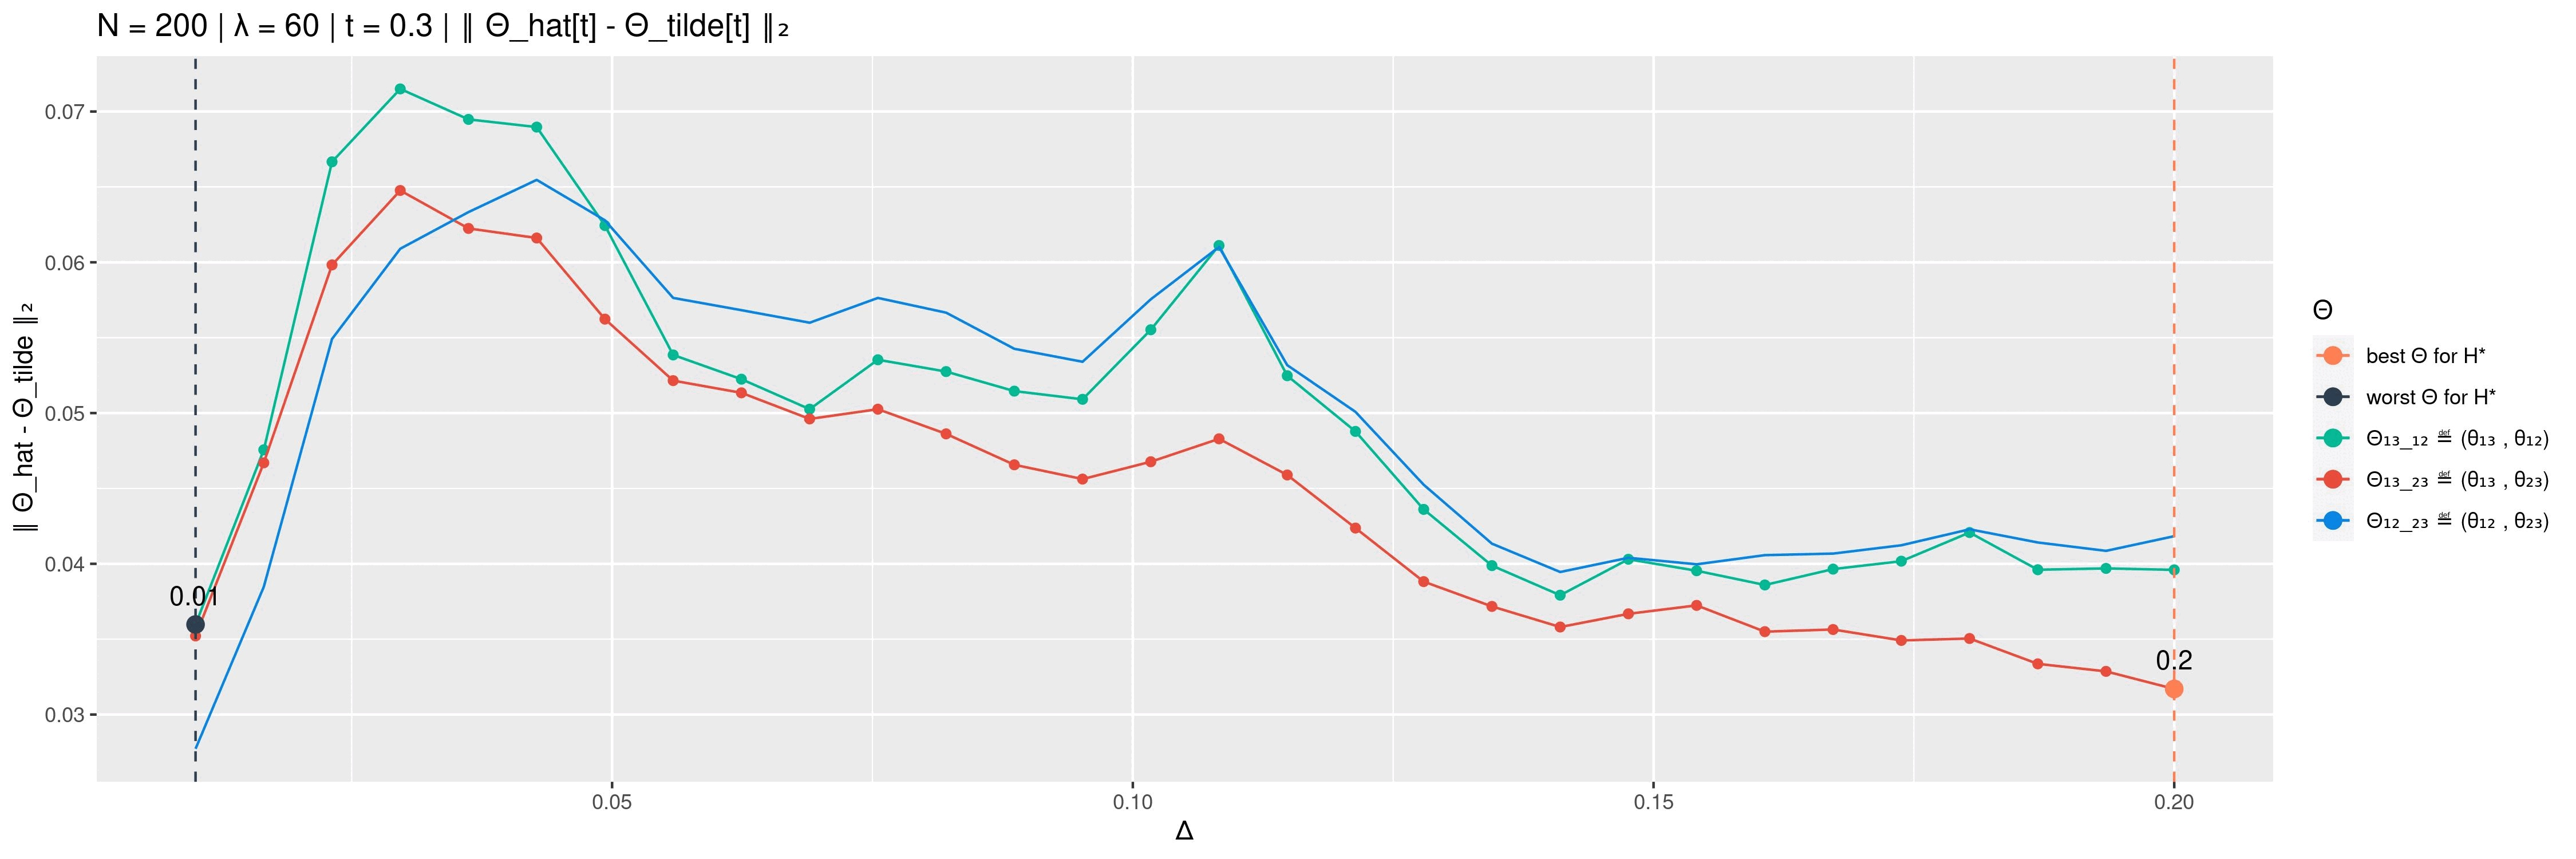
\includegraphics[width=0.8\textwidth]{Images/risque/N200_t0.3_lbd60.jpg}

	Dense :

	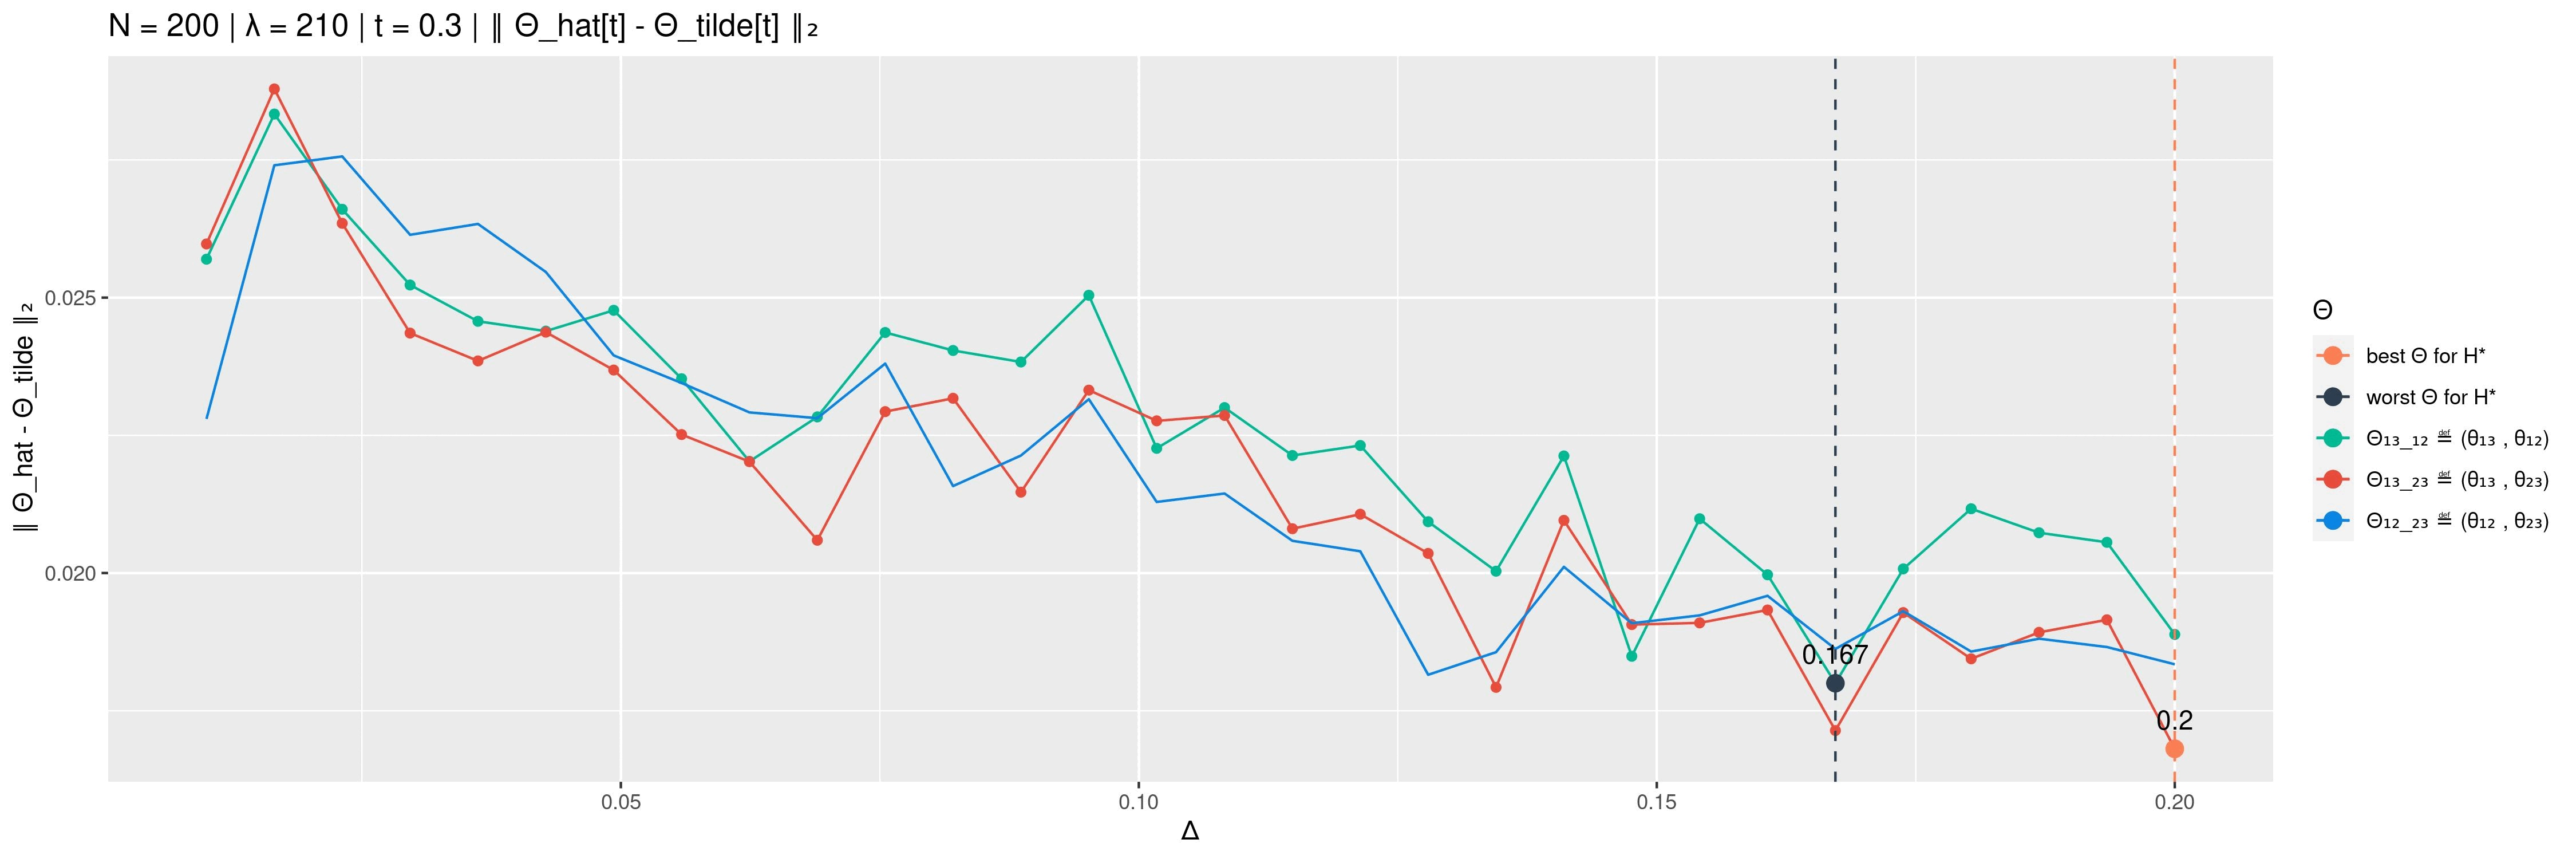
\includegraphics[width=0.8\textwidth]{Images/risque/N200_t0.3_lbd210.jpg}
\end{figure}

\begin{figure}[H]
	\centering
	\textbf{ H = 0.6 }

	Sparse :

	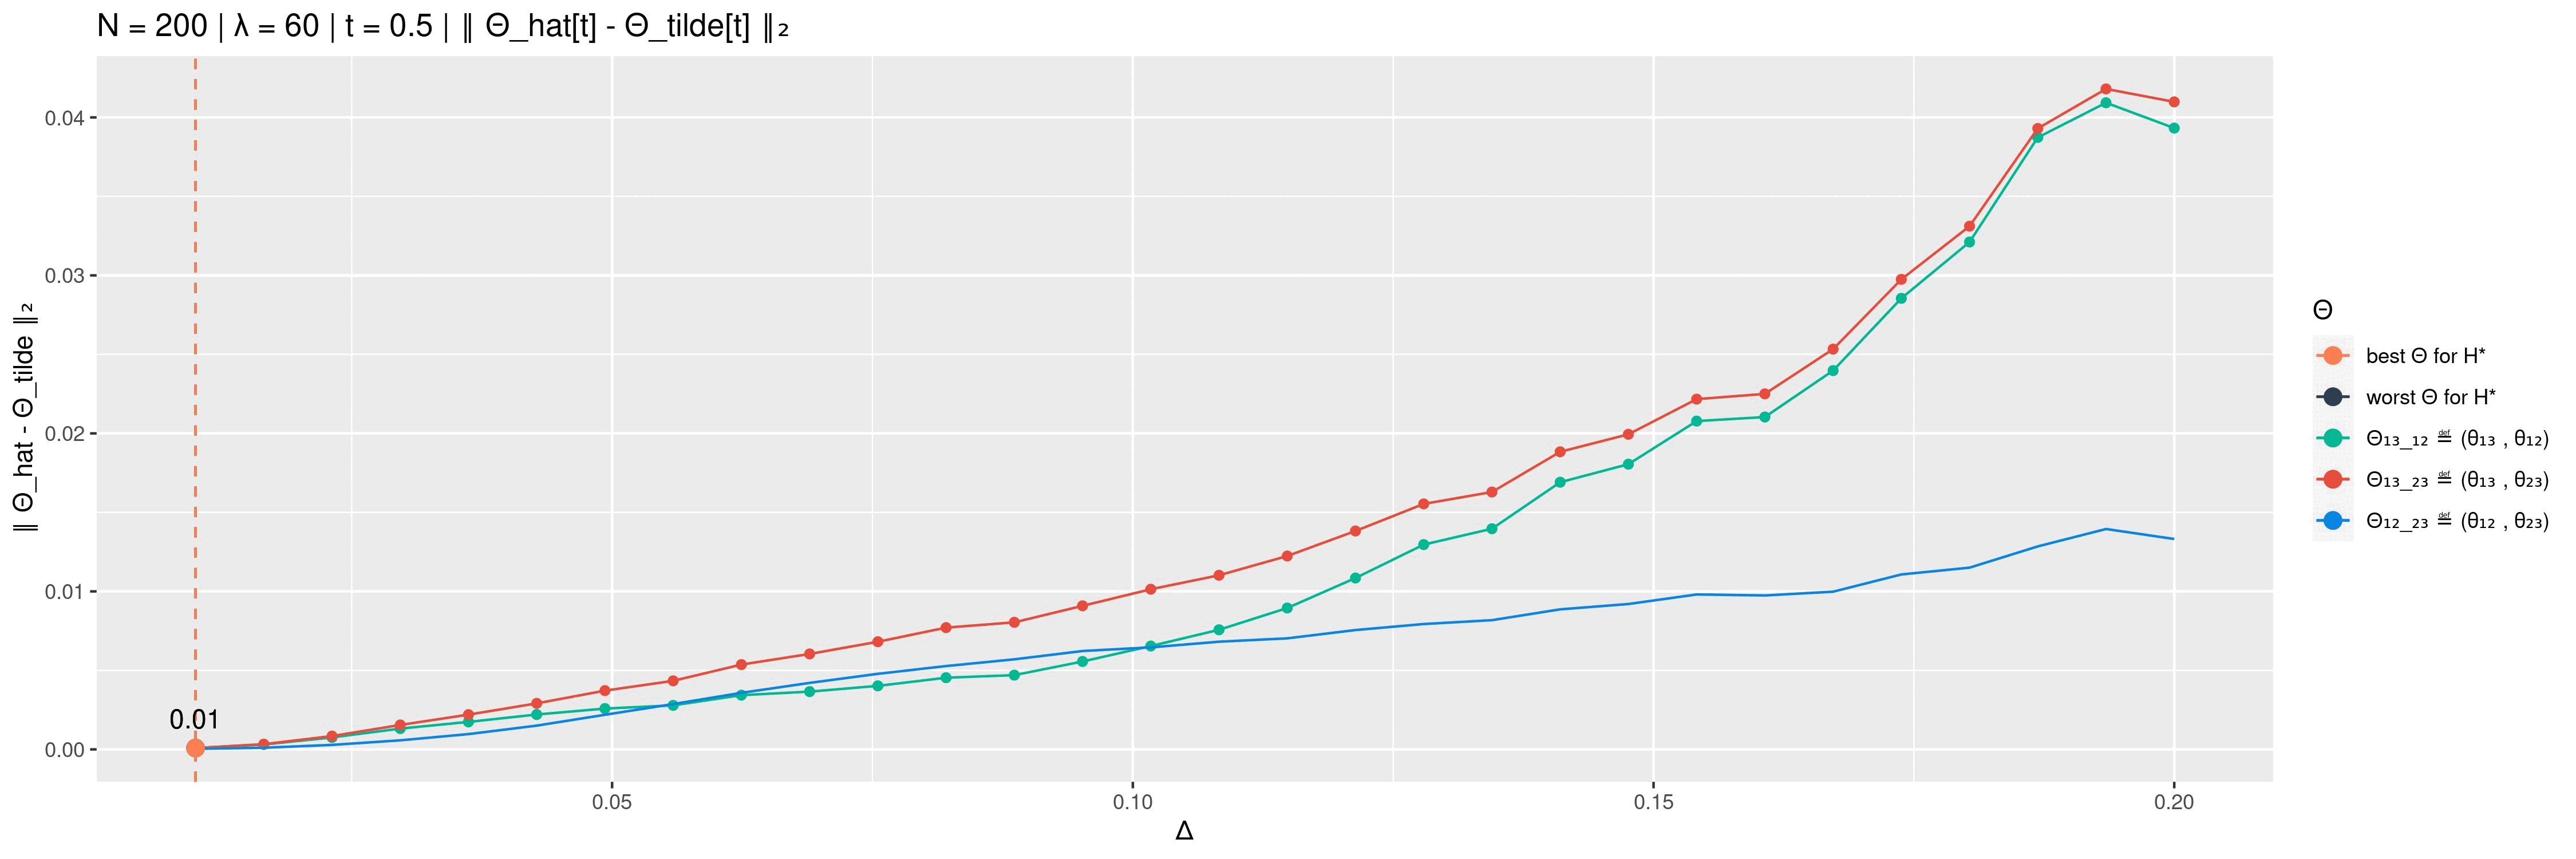
\includegraphics[width=0.8\textwidth]{Images/risque/N200_t0.5_lbd60.jpg}

	Dense :

	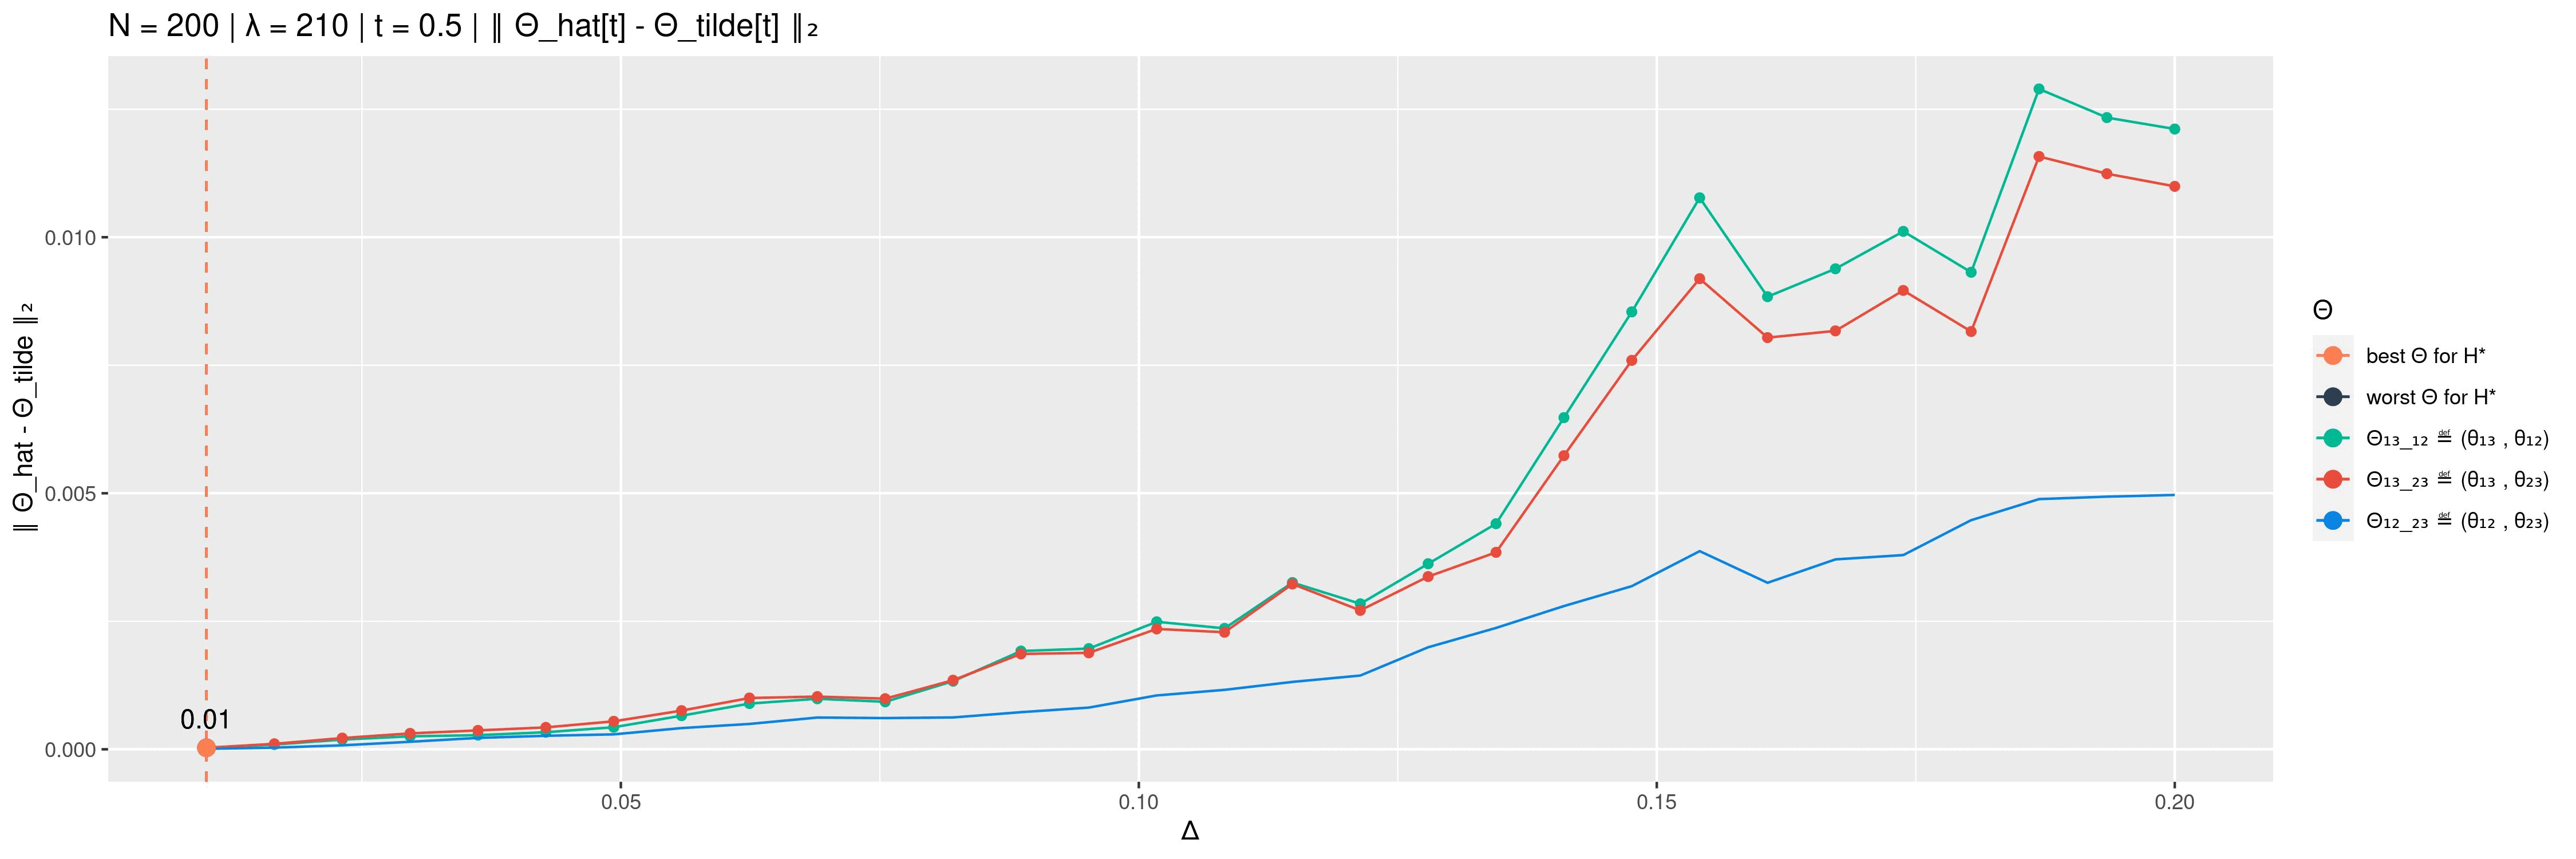
\includegraphics[width=0.8\textwidth]{Images/risque/N200_t0.5_lbd210.jpg}
\end{figure}


\begin{figure}[H]
	\centering
	\textbf{ H = 0.73 }

	Sparse :

	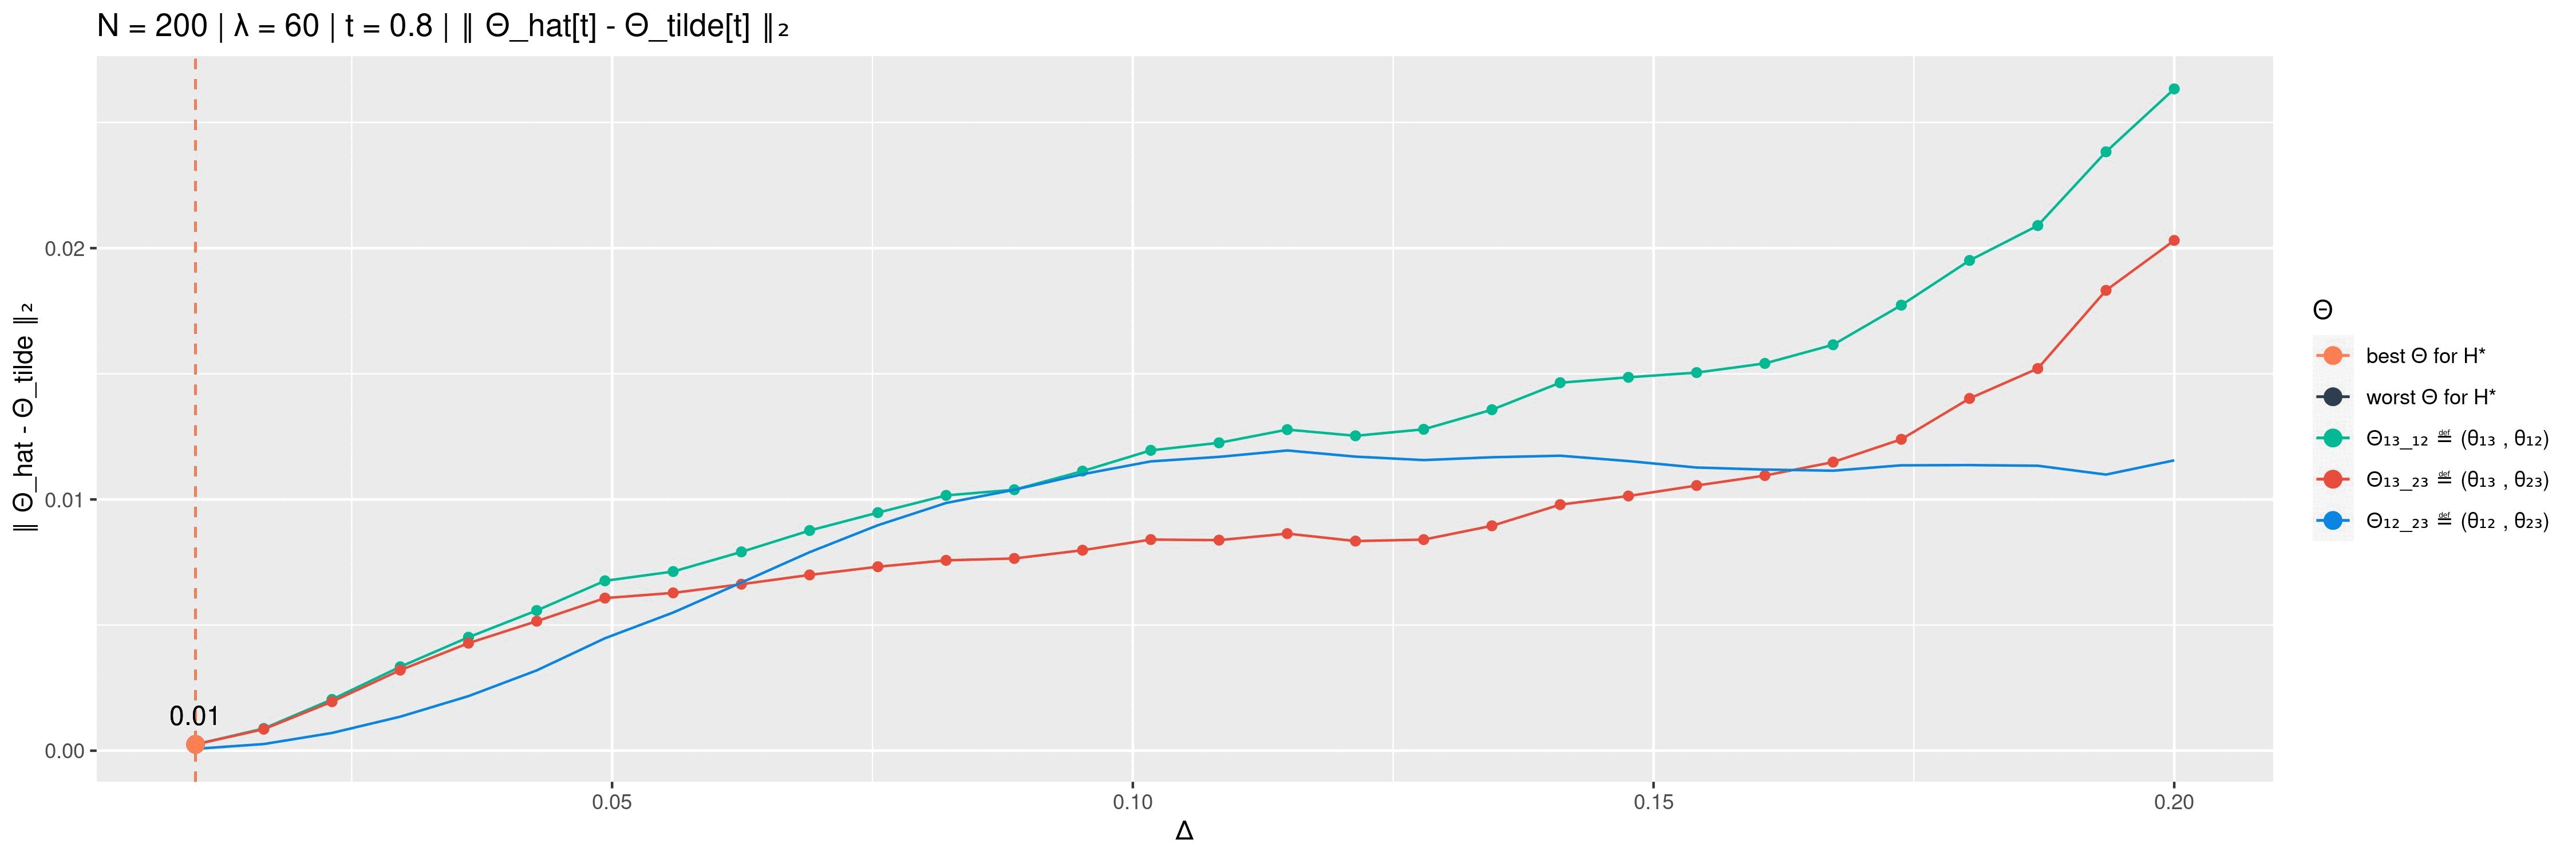
\includegraphics[width=0.8\textwidth]{Images/risque/N200_t0.8_lbd60.jpg}

	Dense :

	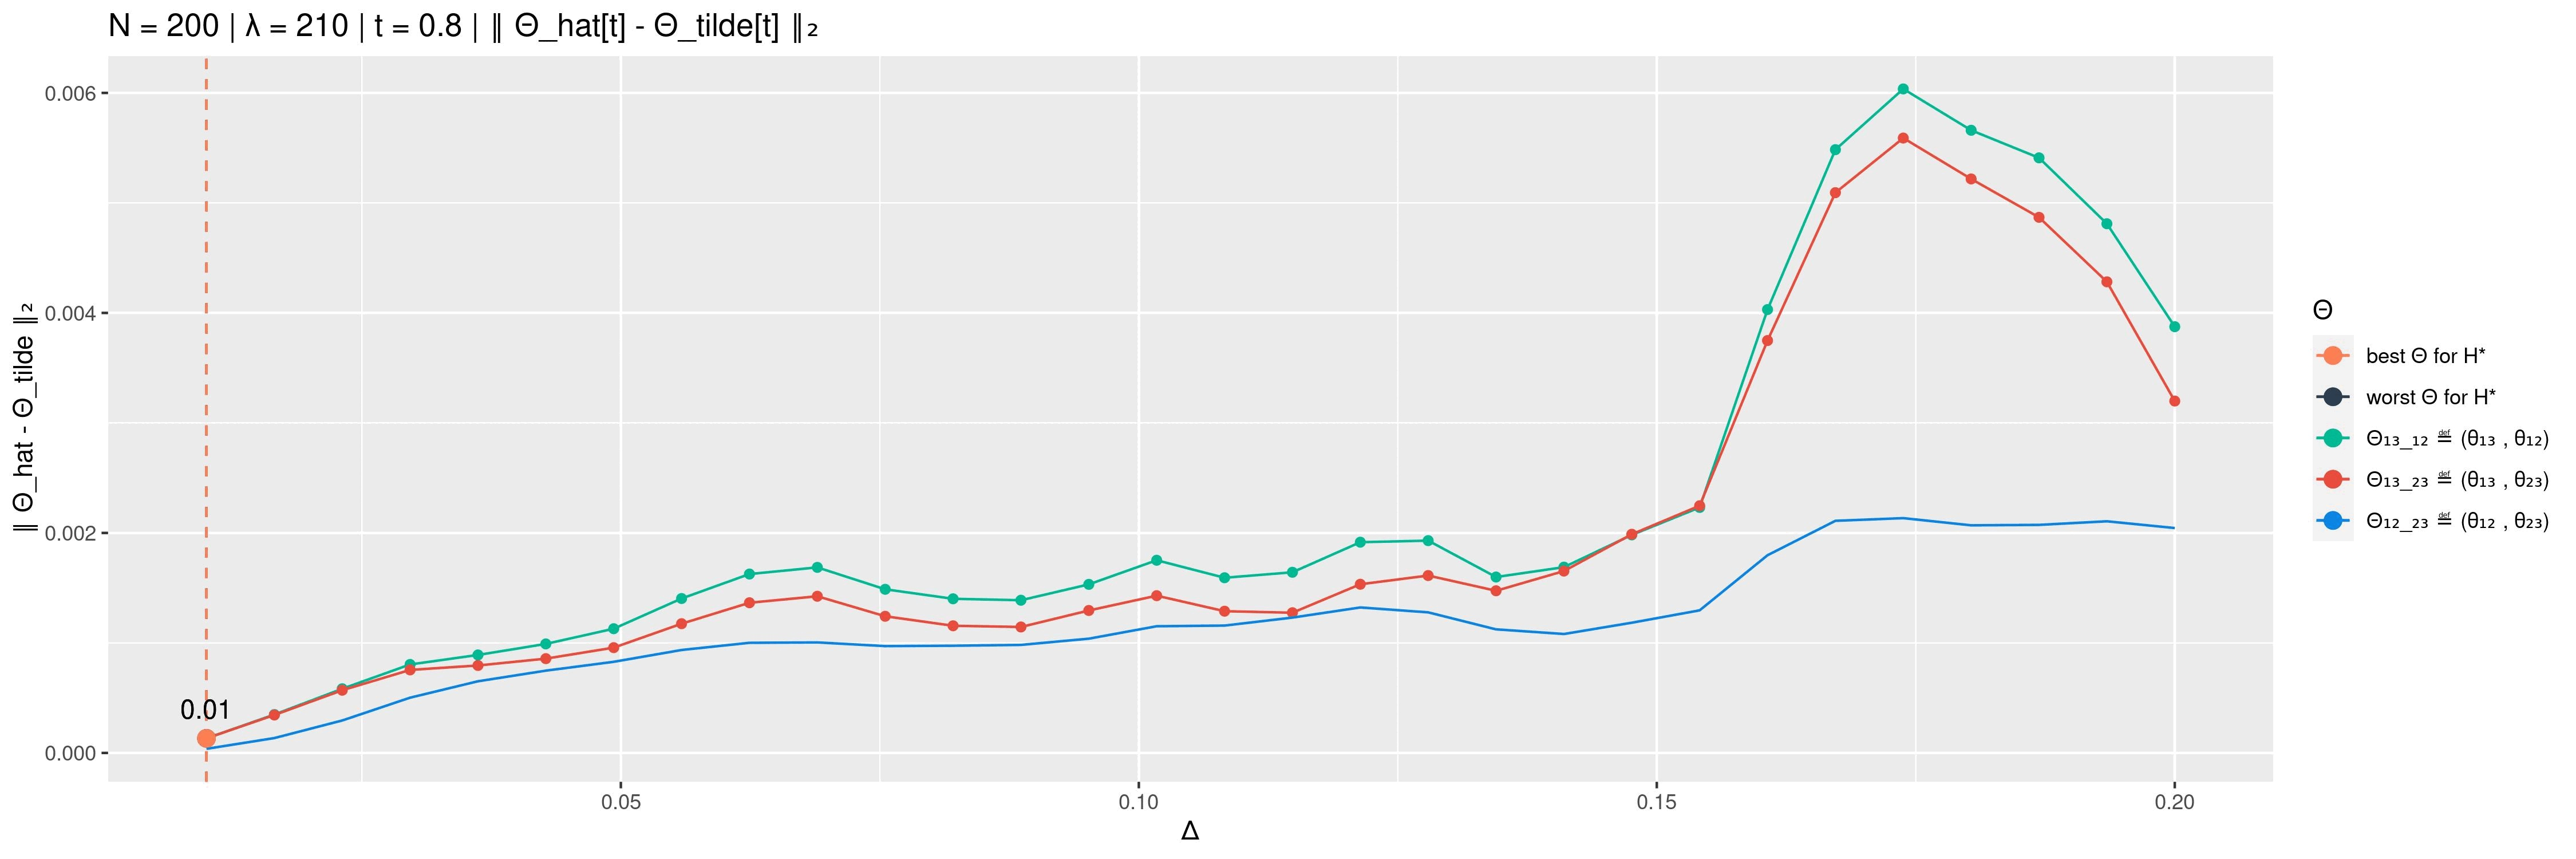
\includegraphics[width=0.8\textwidth]{Images/risque/N200_t0.8_lbd210.jpg}

	\label{fig:sparse_osef}
	\caption{Graphe des risques dans les cas \og sparse \fg et \og raisonnablement dense \fg}
\end{figure}
